\documentclass[acmlarge]{style/acmart}

\usepackage{lipsum}
\usepackage{float}
 
%% \BibTeX command to typeset BibTeX logo in the docs
\AtBeginDocument{%
  \providecommand\BibTeX{{%
    \normalfont B\kern-0.5em{\scshape i\kern-0.25em b}\kern-0.8em\TeX}}}


 \setcopyright{acmcopyright}
 \copyrightyear{2021}
 \acmYear{2021}
 \acmDOI{}


%%
%% These commands are for a JOURNAL article.
 \acmJournal{POMACS}
 \acmVolume{1}
 \acmNumber{1}
 \acmArticle{111}
 \acmMonth{11}

\begin{document}


\title{Wireless Forensics Principles and Investigations}



\author{Evan Lomax}
\email{evn.lmx@gmail.com}
\affiliation{%
  \institution{University of Central Florida}
  \city{Orlando}
  \country{USA}
}

\author{Shenequa Hayes}
\email{shenequa.hayes@gmail.com}
\affiliation{%
  \institution{University of Central Florida}
  \city{Orlando}
  \country{USA}
}
\author{Camilo Lozano}
\email{clozano@knights.ucf.edu}
\affiliation{%
  \institution{University of Central Florida}
  \city{Orlando}
  \country{USA}
}
\author{Shannon Padilla}
\email{JPCharme@gmail.com}
\affiliation{%
  \institution{University of Central Florida}
  \city{Orlando}
  \country{USA}
}

\renewcommand{\shortauthors}{Lomax, et al.}

\begin{abstract}
We will discuss the current and emerging principles and investigations as it pertains to wireless digital forensics. We will look at the past, the present and future of wireless forensics. We will examine the major sub-branches, to include: 802.11 network forensics, IoT vulnerabilities, mobile forensics, available wireless security and forensics software tools. We will compare and contrast some of the major forensic tool suites as well as some emerging technologies.
\end{abstract}

%%
%% The code below is generated by the tool at http://dl.acm.org/ccs.cfm.
\begin{CCSXML}
<ccs2012>
   <concept>
       <concept_id>10003033.10003083.10003014</concept_id>
       <concept_desc>Networks~Network security</concept_desc>
       <concept_significance>500</concept_significance>
       </concept>
   <concept>
       <concept_id>10002978.10003014.10003017</concept_id>
       <concept_desc>Security and privacy~Mobile and wireless security</concept_desc>
       <concept_significance>500</concept_significance>
       </concept>
   <concept>
       <concept_id>10002978.10002979.10002983</concept_id>
       <concept_desc>Security and privacy~Cryptanalysis and other attacks</concept_desc>
       <concept_significance>300</concept_significance>
       </concept>
 </ccs2012>
\end{CCSXML}

\ccsdesc[500]{Networks~Network security}
\ccsdesc[500]{Security and privacy~Mobile and wireless security}
\ccsdesc[300]{Security and privacy~Cryptanalysis and other attacks}

%%
%% Keywords. The author(s) should pick words that accurately describe
%% the work being presented. Separate the keywords with commas.
\keywords{networks, security, IOT, 802.11}


%%
%% This command processes the author and affiliation and title
%% information and builds the first part of the formatted document.
\maketitle

\section{Introduction}
%% TODO add more introduction

In this paper we seek to provide a comprehensive overview of the current and emerging wireless security and forensic techniques used today. Wireless forensics is a vast and complex field with a rising demand for expert forensics and security professionals. By taking a deep dive in the field of 802.11 network forensics, IoT vulnerabilities, mobile forensics, and software forensics 

\section{Internet of Things}

A new growing field of devices has sprung up recently with the development and advances of the field of smart homes. These devices usually feature some sort of network connectivity either Wi-Fi or Bluetooth and are considered a form of edge computing. IoT or Internet of Things has been defined as connectable devices and sensors that allow for remote monitoring and manipulation. In a way they are considered a form of edge computing. The biggest rise in these IoT devices has been in the consumer applications smart home sector where it has really taken off in the years between 2008 and 2009 \cite{evans_iot_2011}.

The ever increasing presence of these IoT devices present a new concern as they are a prone vector for security vulnerabilities. Specially so because of the preferences for manufacturers and consumers to turn to a Wi-Fi internet solution for connecting their devices to outside. With little to no regulation, or even certifications, on how these devices can be implemented it has left a big hole in the market making it difficult to know what to trust. 
% Summary for this section might edit later
In this section we will talk about known big security exploits that have already occurred, best practices to follow, and talk about existing forensic methods that can be used to investigate these vulnerabilities.


\subsection{Background}

One of the big issues mentioned is the low level of security that is present in the IoT devices. One of the reasons they are such a threat is the current trend for these devices is to be individually connected to the internet. Initial implementations of smart home appliances relied more on a hub model where the devices were connected to a central hub. This meant that the devices were not connected to the internet and therefore had no way to communicate with the outside world except through the hub. The idea is to just expose one device to the internet and attempt to secure that one as much as possible. With the rise of cheaper micro controller boards that had built in Wi-Fi, specially the ESP8266, the standard model changed and it became more common to have each individual device connected to the main access point. One of the biggest benefits to this model is also one of its drawbacks; allowing consumers to have multiple different ecosystems. This means that there is even more potential for security attacks as each device can be from a different vendor that may or may not be secured.  

The problem becomes that in a race to the bottom of prices it has lead to corner cutting on the software side to just serve the minimum purpose without insuring any protection. We'll follow up with a couple of known intrusions that have occurred ranging from small mistakes to major security concerns. 


\subsection{Tapplock Smart Lock}

In 2018 smart device manufacturer Tapplock began selling a \$100 smart lock, mean to be a sort of gym locker lock that would allow for unlocking with a fingerprint, with a solid steel construction it also had a mobile app that would allow for unlocking the lock over Bluetooth Low Energy (BLE).
On first glance the lock boasted an 'AES 128-bit encryption', but forensic experts quickly started finding some flaws in its implementations. According to the team, they went from obtaining the lock to completely defeating its security in a mere 45 minutes! \cite{Ken_2018}

What they did was manually pair the BLE device to their computer in which they could then use a tool like Wireshark to sniff the traffic between the lock. To their surprise the lock was using HTTP API requests to control the lock over plaintext. This was the first major red flag, this means anyone able to intercept or be in the middle of the communication would be able to sniff and replicate packets to control it. 

The way they were 'securing' their requests was by using some random data attached to the request. The problem was that it was the same random data on each request, meaning that it was a symmetric key. Knowing this allows can allow for any payload for it to be sent.
Additionally another feature of the app allows for the user to share temporarily access to a guest, but as it turns out the key that you share is the same master key as the user. So even though you can set an expiration date for the guest, they essentially have access to the whole security.

The biggest revelation came from a dumping of code on the chip which revealed how the encryption key was being generated. It generates a hash based of some seed value, which turns out is just the MAC address as a string of the BLE devices, which is the only piece of data that is available to the an attacker!
This was then automated to be used in an app which would scan for nearby BLE devices and identify those that were a Tapplock device then use its MAC address to generate a key and unlock the key. Meaning that anyone with a phone in range of a Tapplock device can unlock it in less than a a couple seconds!

\subsection{Mirai Malware}

One of the most common type of internet based attacks is a Denial-of-Service (DoS) attack. This is when a malicious user or group of users is able to flood a server with requests and cause it to crash. Usually the way to prevent his is by having a firewall in place that blocks all traffic from the attacker. This is done by identifying some sort of pattern in the traffic and blocking it. An advanced form of this attack is a Distributed DoS (DDoS), which consists of a coordinated attacked by many with varying ranging IPs that would be much harder to identify and block. 

In 2016 a botnet malware started to randomly appear. A large amount of CCTV, routers and other IoT devices were being compromised by this malware. It was specially hard to detect as the IoT devices remained mostly fine except for every now and them some sluggishness every and increased bandwith. What was interesting is that this malware is that it is not complex in its nature. What it does once a device is infected is randomly scan for IPs and attempt to ping them on certain known ports. The developer compiled a list of known manufacturers default ports, usernames and passwords. Each node then just attempts pinging until it finds an open device, then its IP is uploaded to a controller that then contacts the other nodes to try to authenticate on the known device until eventually some are compromised by their default passwords. 

Once inside on a compromised device, the malware installs itself on the new device and continues to propagate. This allowed the malware to scale massively. This was then used to DDoS a bunch of websites, including a OVH (one of France's largest hosting companies), Dyn (a DNS provider), and even a cyber security journalist. At its peak there was a recorded bandwidth hitting 1 Tbit/s!\cite{Hertzberg_Mirai_2016}

Most interestingly the was that the source code of the malware was eventually leaked and the creator was identified! Apparently the author had a IT security company that offered protection against DDoS. In a way they were running a protection racket, initially starting with Minecraft servers.

This attack revealed how major manufacturers were using default credentials and allowing easy exploitable security issues. Since the code has been open sourced others have taken to fork it and adapt the same concept to different devices.

\subsection{Best Practices}

As demonstrated from above 

\section{802.11 and Mobile Forensic Tools}

802.11 or “WiFi” has become normal not only in the workplace but also at home. Because of the common use of this technology, it has become necessary to develop tools and techniques in order to conduct forensic investigations on WiFi networks. These tools can simply be used to monitor traffic to find out why a network may be running slower than normal or they can be utilized for in-depth investigations because of an attack. There are also several tools and techniques for attackers or hackers to utilize in order to inject malicious packets, intercept packets, and crack network passwords in order to gain unauthorized access to a wireless network. 
There are several avenues for an examiner to conduct a forensic investigation into a wireless network. The first is examining frames on the network and capturing network traffic or packets utilizing tools and hardware. This will allow the examiner to inspect communications between stations. Packets can also contain clear-text data if unencrypted or if the encryption key is known. Most WiFi networks will typically operate in either 2.4GHz or 5 GHz radio frequency ranges. WiFi ranges are broken down into smaller bands called channels. 2.4GHz band will have 11 channels and 5GHz band will have 45 different channels. 
Wireless Access Points (WAP) can also contain fruitful information for a forensic examiner. WAPs can contain stored logs which will illuminate connections whether they were successful or not. The logs could also contain data about the attempted or successful connection such as IP and MAC addresses as well as timestamps. 
%Below is a screenshot example of a wireless log from a WAP:

\begin{figure}[H]
  \centering
  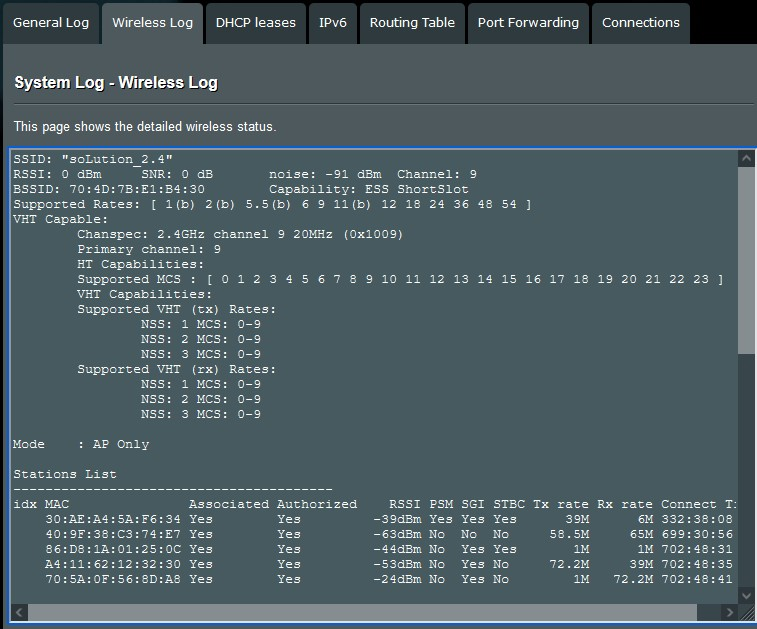
\includegraphics[width=0.5\linewidth]{imgs/waplog.jpg}
  \caption{Screenshot of a wireless log from a WAP}
  \label{fig:waplog}
\end{figure}

This particular log shows real-time connections which can be volatile. Forensic examiners can use real-time logs to determine if an unauthorized client is connected but historic logs can obviously be extremely useful as well. 

\subsection{Wireshark}

In order to an examiner to capture network traffic, an 802.11 wireless card with “monitor mode” capability is required. Wireshark is a useful tool and probably the most used by forensic examiners for monitoring network traffic live and examining historic pcap files. Wireshark allows the examiner to analyze traffic and filter exactly what they are looking for. 
%Below is a screen shot of a live capture using Wireshark:

\begin{figure}[H]
  \centering
  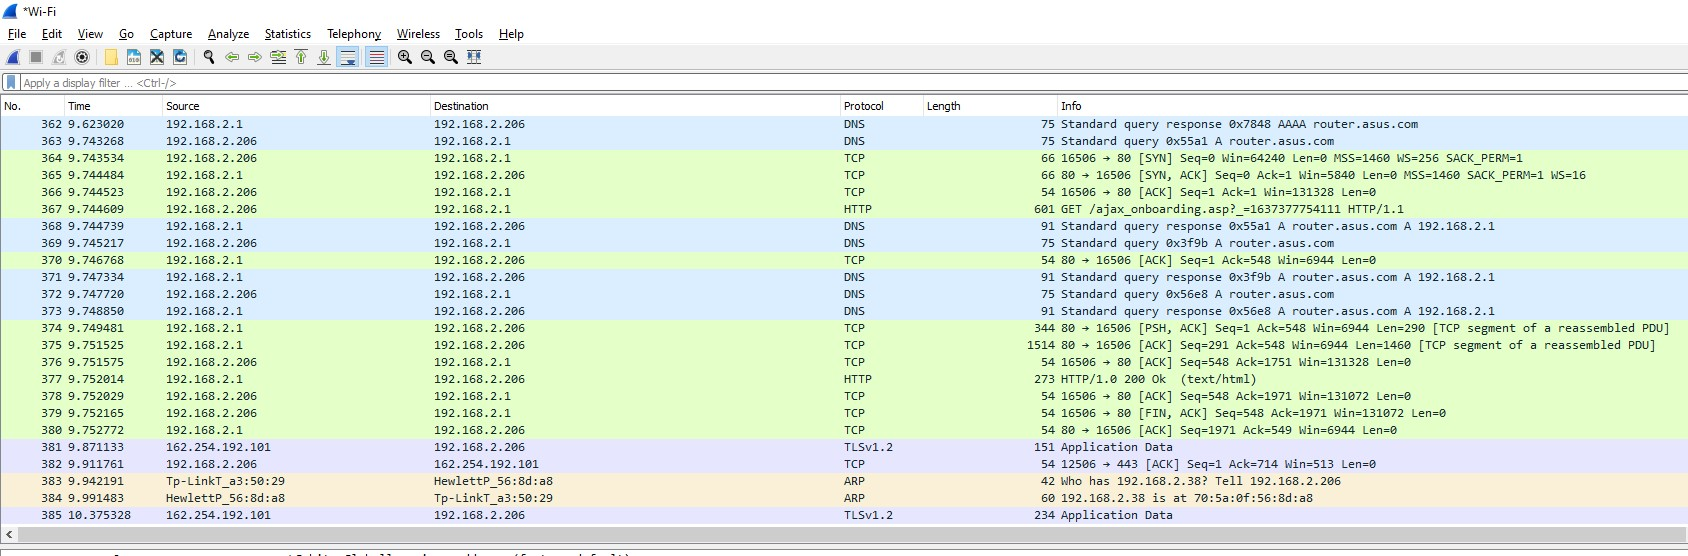
\includegraphics[width=0.5\linewidth]{imgs/wireshark.jpg}
  \caption{Screenshot of Wireshark log}
  \label{fig:wireshark}
\end{figure}

Wireshark displays tons of data on each packet to include packet number of the capture, source IPs, destination Ips, protocols, frame information, mac addresses and packet data. 

\subsection{Snort}

Snort is another tool that can be utilized by an examiner to analyze network traffic. Snort is different from Wireshark in the fact that it can also be used as an Intrusion Protection System. Snort is a type of tool that an enterprise client would likely use such as a network administrator for a company. Snort can alert users of malicious packets set by rules and also log packets for historic analysis. 
%Below is a screenshot of the Snort interface:

\begin{figure}[H]
  \centering
  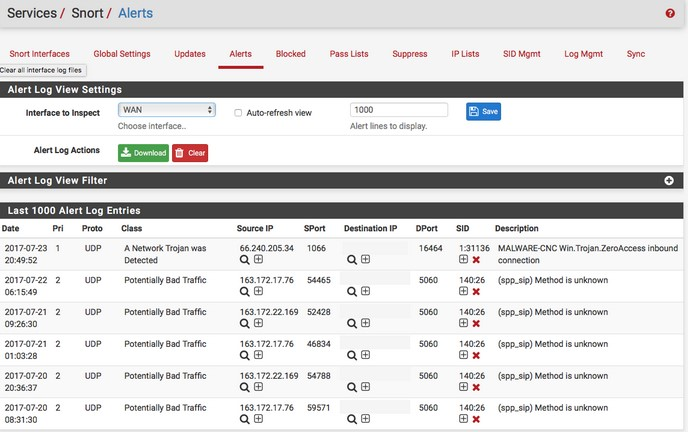
\includegraphics[width=0.5\linewidth]{imgs/snort.jpg}
  \caption{Screenshot of Snort interface}
  \label{fig:snort}
\end{figure}

\subsection{Engage}

Several tools that examiner utilize in 802.11 forensics can also be used be attackers for malicious purposes. One such tool is the Engage Packet Builder tool. The Engage Packet Builder tool allows the user to create/inject packets and most notable allows the user to be able to spoof their IP address to become anonymous. This tool can be used for DOS type attacks. 
%Below is a screenshot from the Engage Packet Builder tool’s interface:

\begin{figure}[H]
  \centering
  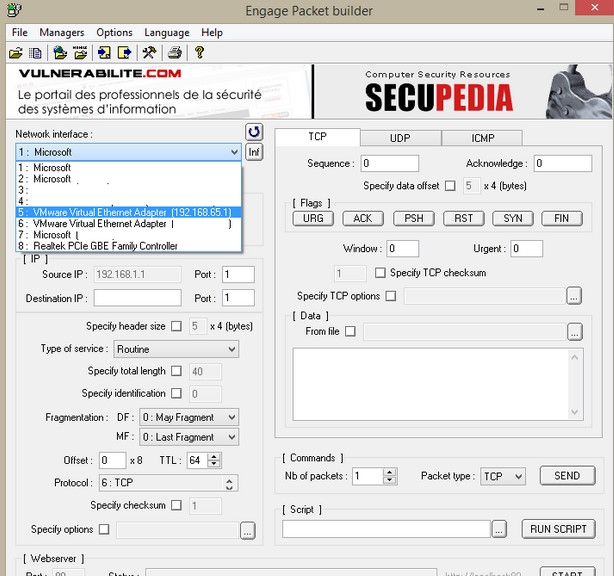
\includegraphics[width=0.5\linewidth]{imgs/engage.jpg}
  \caption{Screenshot of the Engage Packet Builder tool's interface}
  \label{fig:engage}
\end{figure}

\subsection{Aircrack}

Attackers can also utilize Wireshark and a tool called Aircrack-ng in order to crack a WAP’s password. An attacker can sniff out packets with a capable wireless card and capture them utilizing Wireshark. If the attacker is able to capture the correct type of packets, then they can use Aircrack-ng to brute force crack the password. Once the attacker has the encryption password then they can see the data behind all of the packets which could be sensitive data the authorized user of the network does not want to share. 
%Below is a screenshot of an example of Aircrack-ng cracking a password utilizing a brute force method:

\begin{figure}[H]
  \centering
  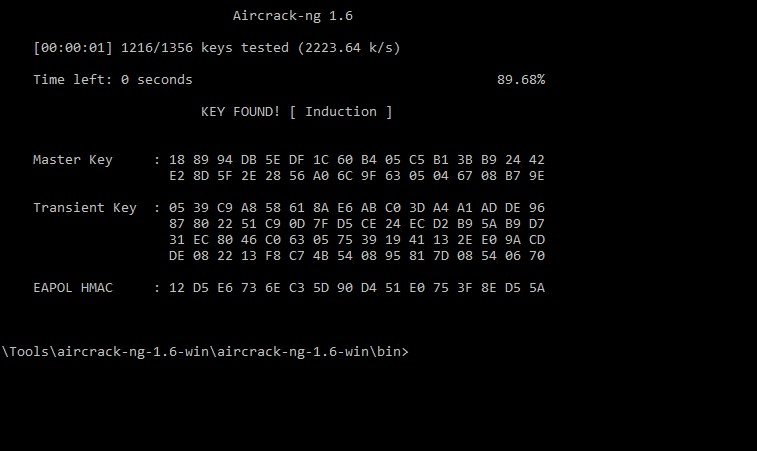
\includegraphics[width=0.5\linewidth]{imgs/aircrack.jpg}
  \caption{Screenshot of the Engage Packet Builder tool's interface}
  \label{fig:aircrack}
\end{figure}

\subsection{Universal Forensic Extraction Device}

“The term “mobile devices” encompasses a wide array of gadgets ranging from mobile phones, smartphones, tablets, and GPS units to wearables and PDAs” \cite{Kostadinov_2019}. Similarly to WiFi, mobile devices have become part of the everyday norm for people. A person can usually not go more than 10 minutes without checking their mobile phone unless they are asleep. Mobile devices such as cell phone can contain a ton of personal information, from banking information to passwords and because of that, mobile devices are a key in some investigations and a target for attackers. 
UFED (Universal Forensic Extraction Device) by Cellebrite is a powerful licensed tool for mobile forensics that allows an investigator to bypass pattern, password or PIN locked devices on both Android and iOS devices, collect data from phones, SIM cards, SD cards, GPS devices, and access data from a variety of different apps. 
%Below is a screenshot of one of the UFED menu lists:

\begin{figure}[H]
  \centering
  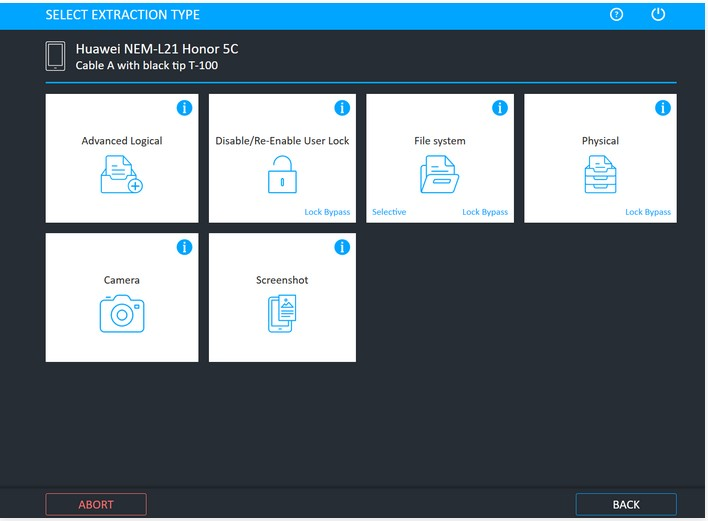
\includegraphics[width=0.5\linewidth]{imgs/ufed.jpg}
  \caption{Screenshot of the UFED menu lists}
  \label{fig:ufed}
\end{figure}

\subsection{iOS Forensic Toolkit}

For iOS specific forensics, the Elcomsoft iOS Forensic Toolkit is extremely useful. This tool can extract all of the data on an iOS device to include, backups, crash logs, media, shared files and can automatically disable screen lock once a device is connected. This tool will work with and iOS device including Apple watches and TV. %Below is a screenshot of the iOS Forensic Toolkit’s main menu:

\begin{figure}[H]
  \centering
  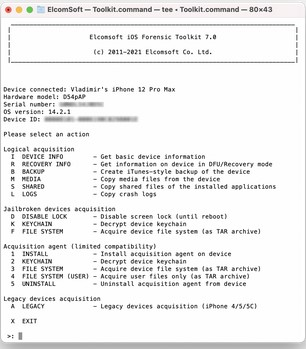
\includegraphics[width=0.5\linewidth]{imgs/ftk.jpg}
  \caption{Screenshot of iOS Forensic Toolkit’s main menu}
  \label{fig:ftk}
\end{figure}

\subsection{Oxygen}

Oxygen Forensic Detective is another powerful tool for mobile forensics. This tool is not only useful for cell phones, but also useful for conducting forensics on IoT devices, device backups, UICC and media cards, drone, and cloud services. It has similar capabilities to the last two mobile forensic tools discussed in that it can bypass screen locks and then extract data. 
%Below is a screenshot of Oxygen Forensic Detective:

\begin{figure}[H]
  \centering
  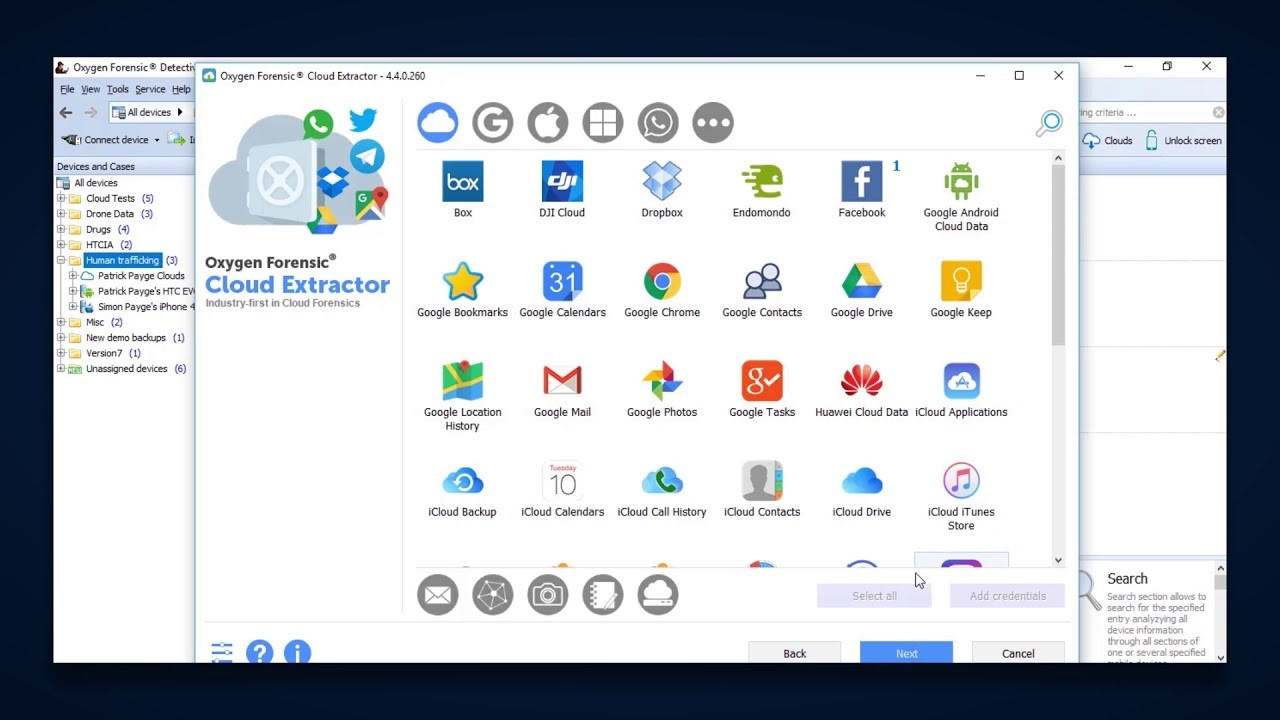
\includegraphics[width=0.5\linewidth]{imgs/oxygen.jpg}
  \caption{Screenshot of Oxygen Forensic Detective}
  \label{fig:oxygen}
\end{figure}
 
Overall, this was just a small sample size of the available tools for that can be used for 802.11 and mobile forensics. There are several different vendors that supply a variety of forensic tools that can be used for law enforcement, government agencies and if in the wrong hands can be used by attackers. As technology becomes more unadvanced and encryption methods become harder to bypass, tools will continue to have to be upgraded or developed in order to keep up with the ability to conduct successful sound evidence.

\section{Conclusion}
%% TODO add conclusion

\bibliographystyle{style/ACM-Reference-Format}
\bibliography{references}

\end{document}
\endinput
%%
